\chapter{Тестирование системы формирования CAPAs на основе изменений репозитория кода} \section{Введение}
В ходе тестирования проверяется работоспособность разработанного инструментария и выполняются поставленные в работе задачи. Основными целями данного этапа являются:
\begin{itemize}
	\item Проверка корректности функционирования пользовательского интерфейса и всех компонентов системы (сбора данных, анализа репозиториев, генерации рекомендаций).
	\item Оценка качества работы классификатора рисковых коммитов на реальных данных, полученных из активных репозиториев.
	\item Тестирование модели генерации CAPA (рекомендаций исправлений) для выявления ошибок и неточностей в алгоритме.
	\item Модульное и нагрузочное тестирование компонентов системы для выявления багов на уровне отдельных модулей и проверки масштабируемости на больших репозиториях.
\end{itemize}
Таким образом, экспериментальное тестирование охватывает проверку как функциональных характеристик (работа интерфейса, правильность алгоритмов), так и нефункциональных (надёжность, производительность) аспектов системы.

\section{Методика проведения тестирования}
Для проверки системы было выбрано несколько тестовых репозиториев с собственными разработками: \texttt{Tq}, \texttt{scherBook}, \texttt{NTO2024-2025}, а также репозитории предоставленные сторонними разработчиками и студентами, которые согласились поучаствовать в тестировании и апробации проекта: \texttt{urlagushka/polytech-labs}, \texttt{urlagushka/h8-pipeline}, \texttt{AlPakh/topotik-backend}, \texttt{AlPakh/topotik-frontend}, \texttt{Pacan4ik/tf-idf}, \texttt{Pacan4ik/tinkoff-course-spring2023}. Эти проекты содержат достаточно разнообразный код (на Java, Python, JavaScript, C++) и различную историю изменений, что обеспечивает репрезентативность данных.

\begin{longtable}{|p{3.5cm}|p{2.2cm}|p{2cm}|p{3cm}|p{4.5cm}|}
	\caption{Описание репозиториев, использованных в тестировании}
	\label{tab:test_repos} \\
	\hline
	\textbf{Репозиторий} & \textbf{Язык(и)} & \textbf{Кол-во коммитов} & \textbf{Тип проекта} & \textbf{Краткое описание} \\
	\hline
	\endfirsthead
	
	\multicolumn{5}{c}{{\tablename\ \thetable{}}} \\
	\hline
	\textbf{Репозиторий} & \textbf{Язык(и)} & \textbf{Кол-во коммитов} & \textbf{Тип проекта} & \textbf{Краткое описание} \\
	\hline
	\endhead
	
	\hline \multicolumn{5}{r}{{}} \\
	\endfoot
	
	\hline
	\endlastfoot
	
	\texttt{urlagushka/
		polytech-labs} & C++, Java & 82 & Учебный проект & Набор лабораторных работ по программной инженерии; содержит решения на нескольких языках. \\
	\hline
	\texttt{urlagushka/
		h8-pipeline} & Python & 110 & ML/AI пайплайн & Инициализатор проекта на базе Hailo SDK; используется для компьютерного зрения. \\
	\hline
	\texttt{Ausland3r/Tq} & Python & 40 & Фреймворк для тестов & Небольшой собственный фреймворк на базе Pytest и Pydantic. \\
	\hline
	\texttt{Ausland3r/
		scherBook} & JavaScript & 39 & Веб-приложе-
		ние & Клиентское приложение для платформы книгообмена; реализован основной UI. \\
	\hline
	\texttt{Ausland3r/
		NTO2024-2025} & Python & 69 & Учебный проект & Материалы к проекту "Умный город" для школьников; используется в рамках NTO. \\
	\hline
	\texttt{Pacan4ik/
		tf-idf} & Python & 36 & Алгоритм обработки текста & Базовая реализация TF-IDF для анализа текстов на русском языке. \\
	\hline
	\texttt{Pacan4ik/
		tinkoff-course-
		spring2023} & Java & 188 & Курсовой проект & Проект на Java Spring Boot с интеграцией Telegram-бота и веб-интерфейсом. \\
	\hline
	\texttt{AlPakh/
		topotik-
		backend} & Python (FastAPI) & 38 & Серверная часть & REST API бэкенд с авторизацией, ORM-моделями и обработкой карт. \\
	\hline
	\texttt{AlPakh/
		topotik-
		frontend} & JavaScript (Vue) & 27 & Клиентская часть & Vue-приложение с маршрутизацией, формами и подключением к API. \\
	\hline
	\texttt{jup-ag/
		pyth-
		crosschain} & Python, Solidity & 3692 & Инфраструк-
		тура Web3 & Форк проекта Jup-ag с доработками Pyth network: кроссчейн модуль для верификации транзакций. \\
	\hline
\end{longtable}

\section{Сравнение моделей классификации}

Для оценки эффективности алгоритмов машинного обучения в задаче предсказания рисковых коммитов был разработан универсальный класс \texttt{CommitRiskModel}. Он предоставляет единый интерфейс к различным классификаторам из \texttt{scikit-learn}, а также \texttt{deep-forest}. Класс реализует методы \texttt{fit()}, \texttt{predict()}, \texttt{predict\_proba()}, \texttt{feature\_importances()} и \texttt{evaluate\_model()}.

Для сравнения были обучены три модели — RandomForest, XGBoost и DeepForest — на выборке коммитов с автоматически определёнными метками риска. Эксперименты проводились как на небольших проектах (в пределах сотни коммитов), так и на объёмном репозитории \texttt{pyth-crosschain} (3692 коммита).


\begin{table}[h!]
	\centering
	\caption{Сравнение моделей классификации на малом и большом репозитории}
	\label{tab:metrics_comparison_combined}
	\resizebox{\textwidth}{!}{
		\begin{tabular}{|l|c c c c|c c c c|}
			\hline
			\multirow{2}{*}{\textbf{Модель}} &
			\multicolumn{4}{c|}{\textbf{Малый проект}} &
			\multicolumn{4}{c|}{\textbf{Большой проект}} \\
			& Precision & Recall & F1-score & ROC-AUC
			& Precision & Recall & F1-score & ROC-AUC \\
			\hline
			RandomForest & 1.000 & 0.500 & 0.667 & 0.983
			& 0.976 & 0.872 & 0.921 & 0.999 \\
			XGBoost      & 1.000 & 0.500 & 0.667 & 1.000
			& 0.958 & 0.979 & 0.968 & 1.000 \\
			DeepForest   & 0.667 & 1.000 & 0.800 & 1.000
			& 0.882 & 0.957 & 0.918 & 0.997 \\
			\hline
		\end{tabular}
	}
\end{table}

\begin{figure}[ht]
	\centering
	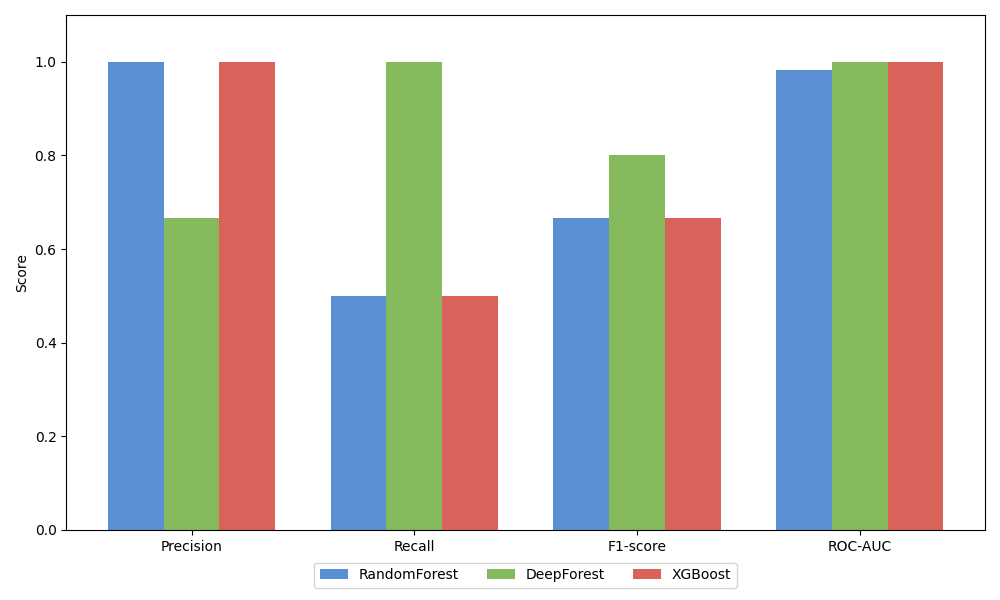
\includegraphics[width=0.85\textwidth]{my_folder/images/low_model_comparison.png}
	\caption{Результаты для разных моделей на малом проекте}
	\label{tab:model_comparison1}
\end{figure}

На малом проекте DeepForest заметно превосходит другие модели по полноте (Recall = 1.0) и F1-score (0.800), что критично в условиях ограниченного количества обучающих примеров. RandomForest и XGBoost в таких условиях оказались переобученными и показали высокую точность, но пропустили половину рисковых коммитов. Это говорит о недостаточной чувствительности традиционных моделей при малом числе объектов.

\begin{figure}[ht]
	\centering
	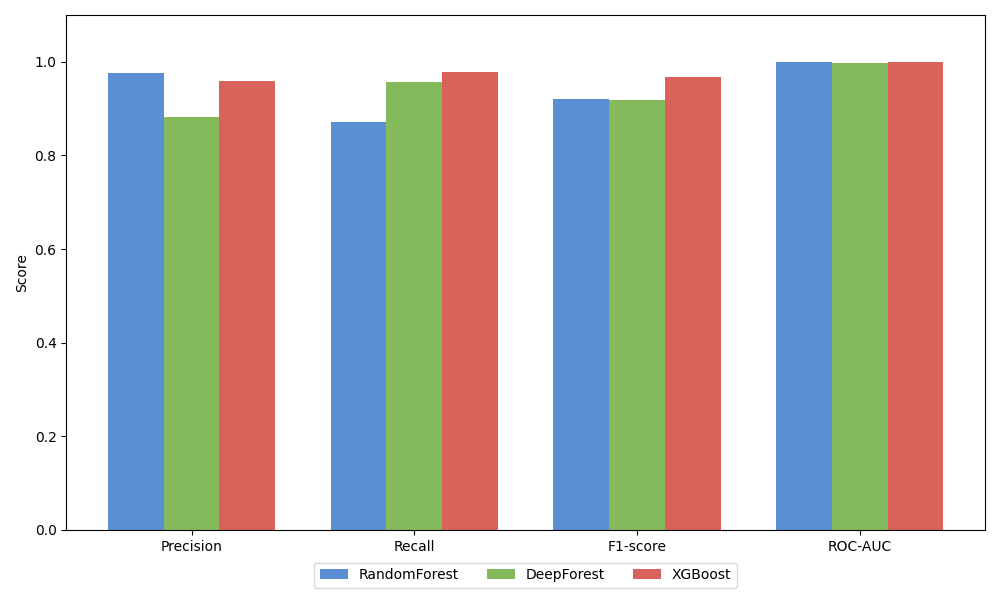
\includegraphics[width=0.85\textwidth]{my_folder/images/high_model_comparison.png}
	\caption{Результаты для разных моделей на большом проекте}
	\label{tab:model_comparison2}
\end{figure}

На большом проекте (\texttt{pyth-crosschain}) ситуация меняется: XGBoost показывает лучшие результаты по F1-мере (0.968) и Recall (0.979), при этом сохраняя приемлемую точность (0.958). RandomForest также демонстрирует хорошее качество, особенно по метрике ROC-AUC (0.999). DeepForest остаётся конкурентоспособным, но немного уступает по F1-score и Precision, что можно объяснить большей сложностью структуры модели и возможным недообучением на шумных данных.

DeepForest оказывается особенно эффективной моделью в условиях малого количества данных, где критично не упустить ни одного рискового случая. Его архитектура каскадных слоёв обеспечивает высокую полноту даже на небольших выборках. Однако при наличии большого объёма данных более устойчивыми и точными оказываются градиентные модели, такие как XGBoost.

Таким образом:
\begin{itemize}
	\item Для небольших проектов с ограниченной историей коммитов предпочтительнее использовать \texttt{DeepForest}, чтобы минимизировать пропущенные риски.
	\item Для крупных репозиториев рекомендуется \texttt{XGBoost} как наиболее сбалансированная и надёжная модель по метрикам качества.
\end{itemize}

В итоге можно с уверенностью сказать, что разработанный унифицированный класс \texttt{CommitRiskModel} позволяет гибко подключать и тестировать разные алгоритмы без необходимости переписывать код, что делает систему легко масштабируемой и адаптируемой под разные сценарии.

\section{Модульное тестирование}

Для обеспечения качества и надёжности разработанного программного обеспечения выполнено модульное тестирование ключевых компонентов системы. В рамках тестирования было создано и выполнено 12 отдельных тестов, охватывающих основные сценарии работы и критичные граничные случаи. Основные направления тестирования и проверяемые аспекты включают:

\begin{itemize}
	\item \texttt{ml\_model.py}:
Проверялись основные методы обучения и предсказания моделей машинного обучения. Тесты, такие как \verb|test_model_extremes_and_balanced_cases| и \verb|test_model_predict_|
\verb|proba_output|, гарантировали корректную работу метода \texttt{fit()}, проверяли способность модели обучаться на реальных и частично неполных данных, а также корректно обрабатывать ситуации с отсутствием или неполнотой входных данных. Валидация предсказаний включала проверку возвращаемых значений — скалярных вероятностей в диапазоне от 0 до 1.

Данный набор тестов помогает своевременно обнаруживать ошибки, связанные с изменениями в логике обучения и предсказания, предотвращая ошибки при работе с моделями машинного обучения.

\item \texttt{repository\_analysis.py}:

Проверялся процесс сбора и обработки статистики по коммитам из репозитория. В тестах, например, \texttt{test\_repository\_empty\_and\_corrupted} были учтены разные ситуации: работа с нормальным репозиторием с несколькими коммитами, а также с пустым репозиторием или с некорректными данными или отсутствующими файлами. Тесты гарантировали, что модуль не выдаёт ошибок при отсутствии данных, а возвращает корректные пустые структуры.  

Это снижает риск сбоев в работе системы при взаимодействии с нестандартными или пустыми репозиториями.

\item \texttt{recommendations.py}: 

Проверялись функции генерации рекомендаций на основе анализа изменений в коммитах. Тест \texttt{test\_recommendations\_extreme\_commit} моделирует ситуации с коммитами без добавленных строк кода, наличием уже существующих рекомендаций. Проверялась корректность формируемых списков рекомендаций.

Это позволяет гарантировать, что рекомендации будут релевантными и не содержат дублирующей или ошибочной информации.

\item \texttt{app.py}:

Этот модуль содержит ключевые функции, обеспечивающие загрузку и анализ данных из репозиториев, обучение модели машинного обучения и обновление табличного представления результатов. Тесты \texttt{test\_load\_and\_analyze\_repos}, \texttt{test\_train\_and\_update\_model} и \texttt{test\_update\_tabs} проверяют корректность выполнения основных операций.
\end{itemize}

Все тесты были автоматизированы с использованием фреймворка \texttt{pytest} и обеспечили покрытие ключевых функциональных частей системы более чем на \verb|75%|. Такой уровень тестового покрытия подтверждает надёжность и стабильность реализации, а также значительно упрощает сопровождение и дальнейшее развитие кода, обеспечивая своевременное выявление регрессий и ошибок.

\begin{figure}[ht]
	\centering
	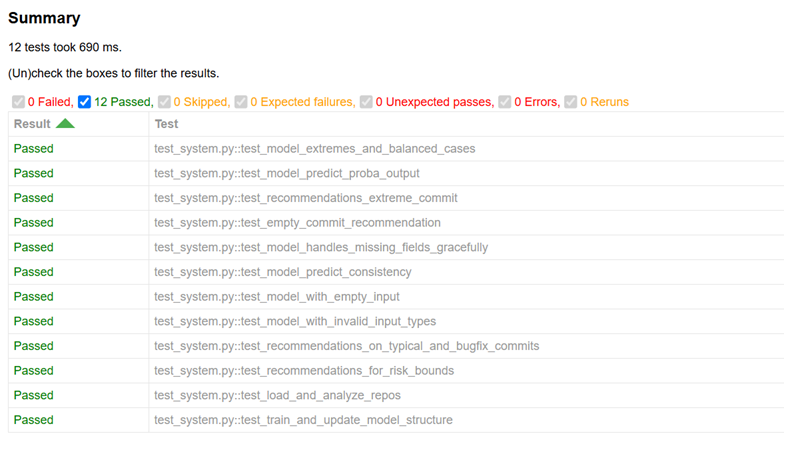
\includegraphics[width=\textwidth]{my_folder/images/test_result.png}
	\caption{Отчёт с результатом прогона автотестов в pytest-html}
	\label{tab:test_pytest}
\end{figure}

\begin{figure}[ht]
	\centering
	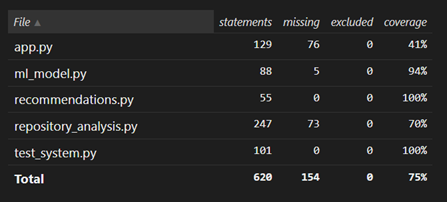
\includegraphics[width=\textwidth]{my_folder/images/coverage.png}
	\caption{Отчёт по покрытию автотестами в pytest-cov}
	\label{tab:test_pytest2}
\end{figure}

\section{Нагрузочное тестирование}

Нагрузочное тестирование проводилось с целью оценки производительности системы при работе с крупными репозиториями. В качестве тестового примера был выбран репозиторий \texttt{jup-ag/pyth-crosschain} с более чем 3000 коммитов. Тестирование выполнялось на машине со следующими характеристиками: процессор AMD Ryzen 9 7900X, 16 ГБ оперативной памяти и SSD-накопитель.

\begin{itemize}
	\item Общее время обработки полного репозитория составило 46 минут. Основная часть времени затрачивается на последовательный запуск статического анализа (Pylint, Checkstyle) для сотен файлов. Дополнительное время уходит на загрузку коммитов через API GitHub, особенно при большом количестве коммитов в репозитории.
	
	\item Наиболее ресурсоёмкой подсистемой оказался статический анализ: последовательный запуск линтеров на большом количестве файлов существенно увеличивает нагрузку на ресурсы компьютера. Максимальная загрузка CPU достигала 53\%, а использование оперативной памяти — до 8 ГБ.
\end{itemize}
Для ускорения работы возможно применение кеширования результатов анализа и параллельной обработки файлов. Для избежания повторной загрузки данных с GitHub система сохраняет локальную копию репозитория. Поскольку API GitHub имеет ограничения по скорости и количеству запросов, локальный клон позволяет минимизировать обращения к API и работать с полной историей и файлами непосредственно на диске, что ускоряет повторный анализ уже загруженных репозиториев. Также чтобы не было необходимости постоянно запускать систему для получения рекомендаций весь список рекомендаций сохраняется локально в md файл и отправляется в отдельную ветку в удаленном репозитории.


В целом система стабильно справлялась с обработкой крупного репозитория, обеспечивая корректные результаты и бесперебойную работу. Максимальная нагрузка приходилась на этап анализа качества кода. Полученные результаты подтверждают, что разработанные компоненты способны эффективно работать с реальными проектами значительных размеров.

\begin{figure}[ht]
	\centering
	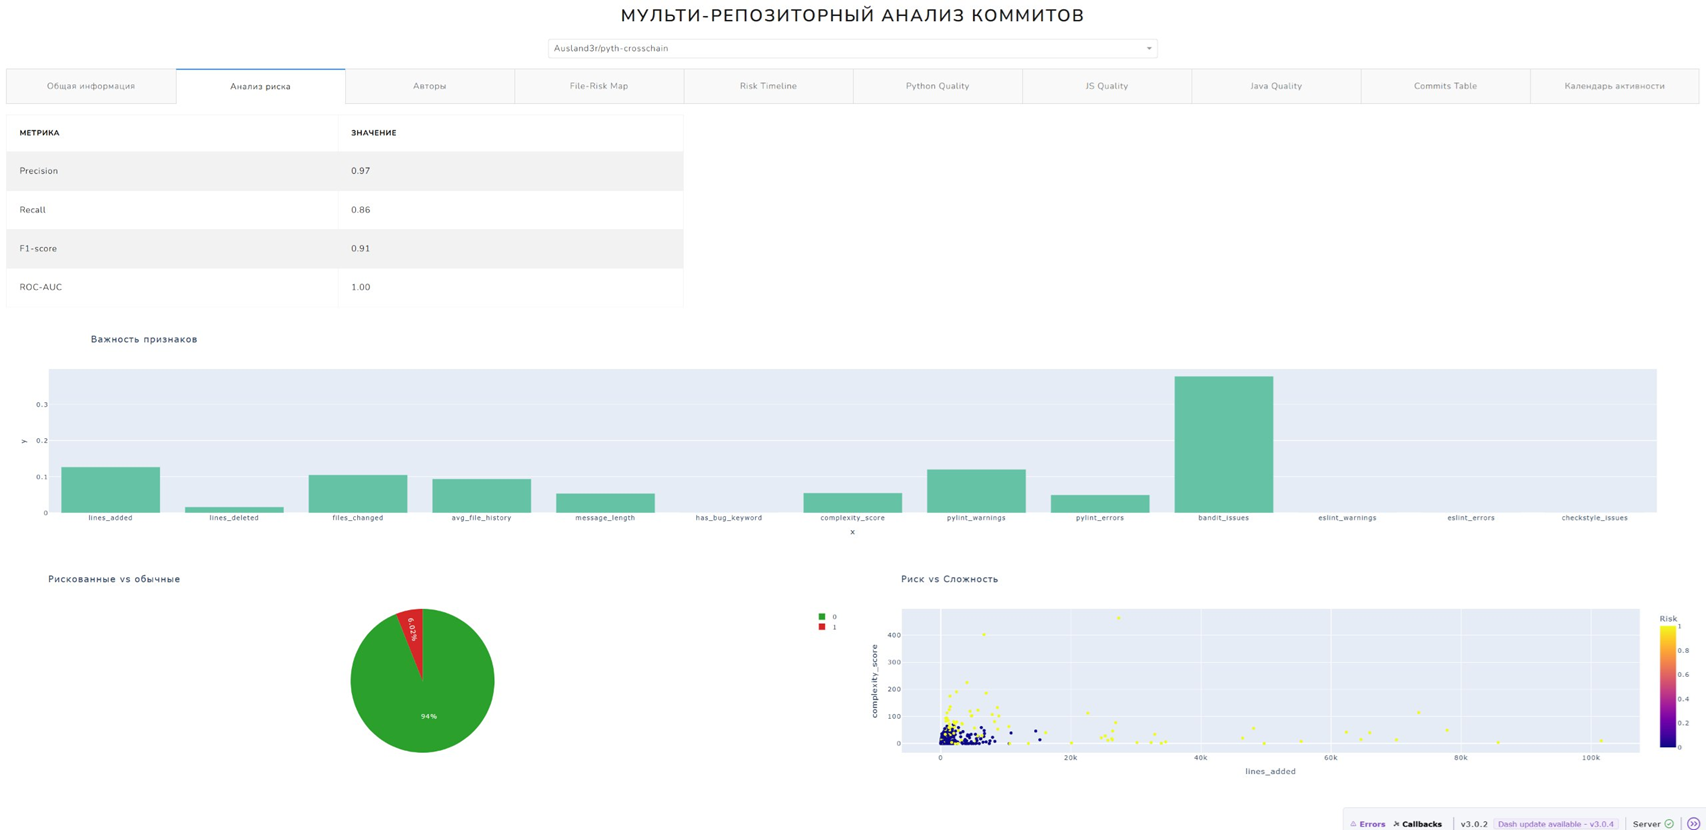
\includegraphics[width=\textwidth]{my_folder/images/nagruzka.png}
	\caption{Запущенная система с репозиторием \texttt{jup-ag/pyth-crosschain}}
	\label{tab:nagruzka}
\end{figure}

\subsection{Обзор и интерпретация результатов}
Визуализация результатов анализа коммитов позволяет быстро выявлять тенденции в проекте. Рассмотрим пример репозитория \texttt{Ausland3r/NTO2024-2025}. На рисунках приведены разные аспекты анализа:

Рисунок~\ref{fig:commit_stats} показывает гистограммы базовых метрик коммитов. Видно, что большинство коммитов содержит меньше 10 добавленных или удалённых строк, а также влияет не более чем на 5 файлов. Сложность изменений (четвёртый график) в большинстве случаев небольшая. Такие диаграммы позволяют визуально оценить, что значительная часть коммитов малых по размеру и сложности, что характерно для аккуратного ведения проекта. 

 \begin{figure}[H]
	\centering
	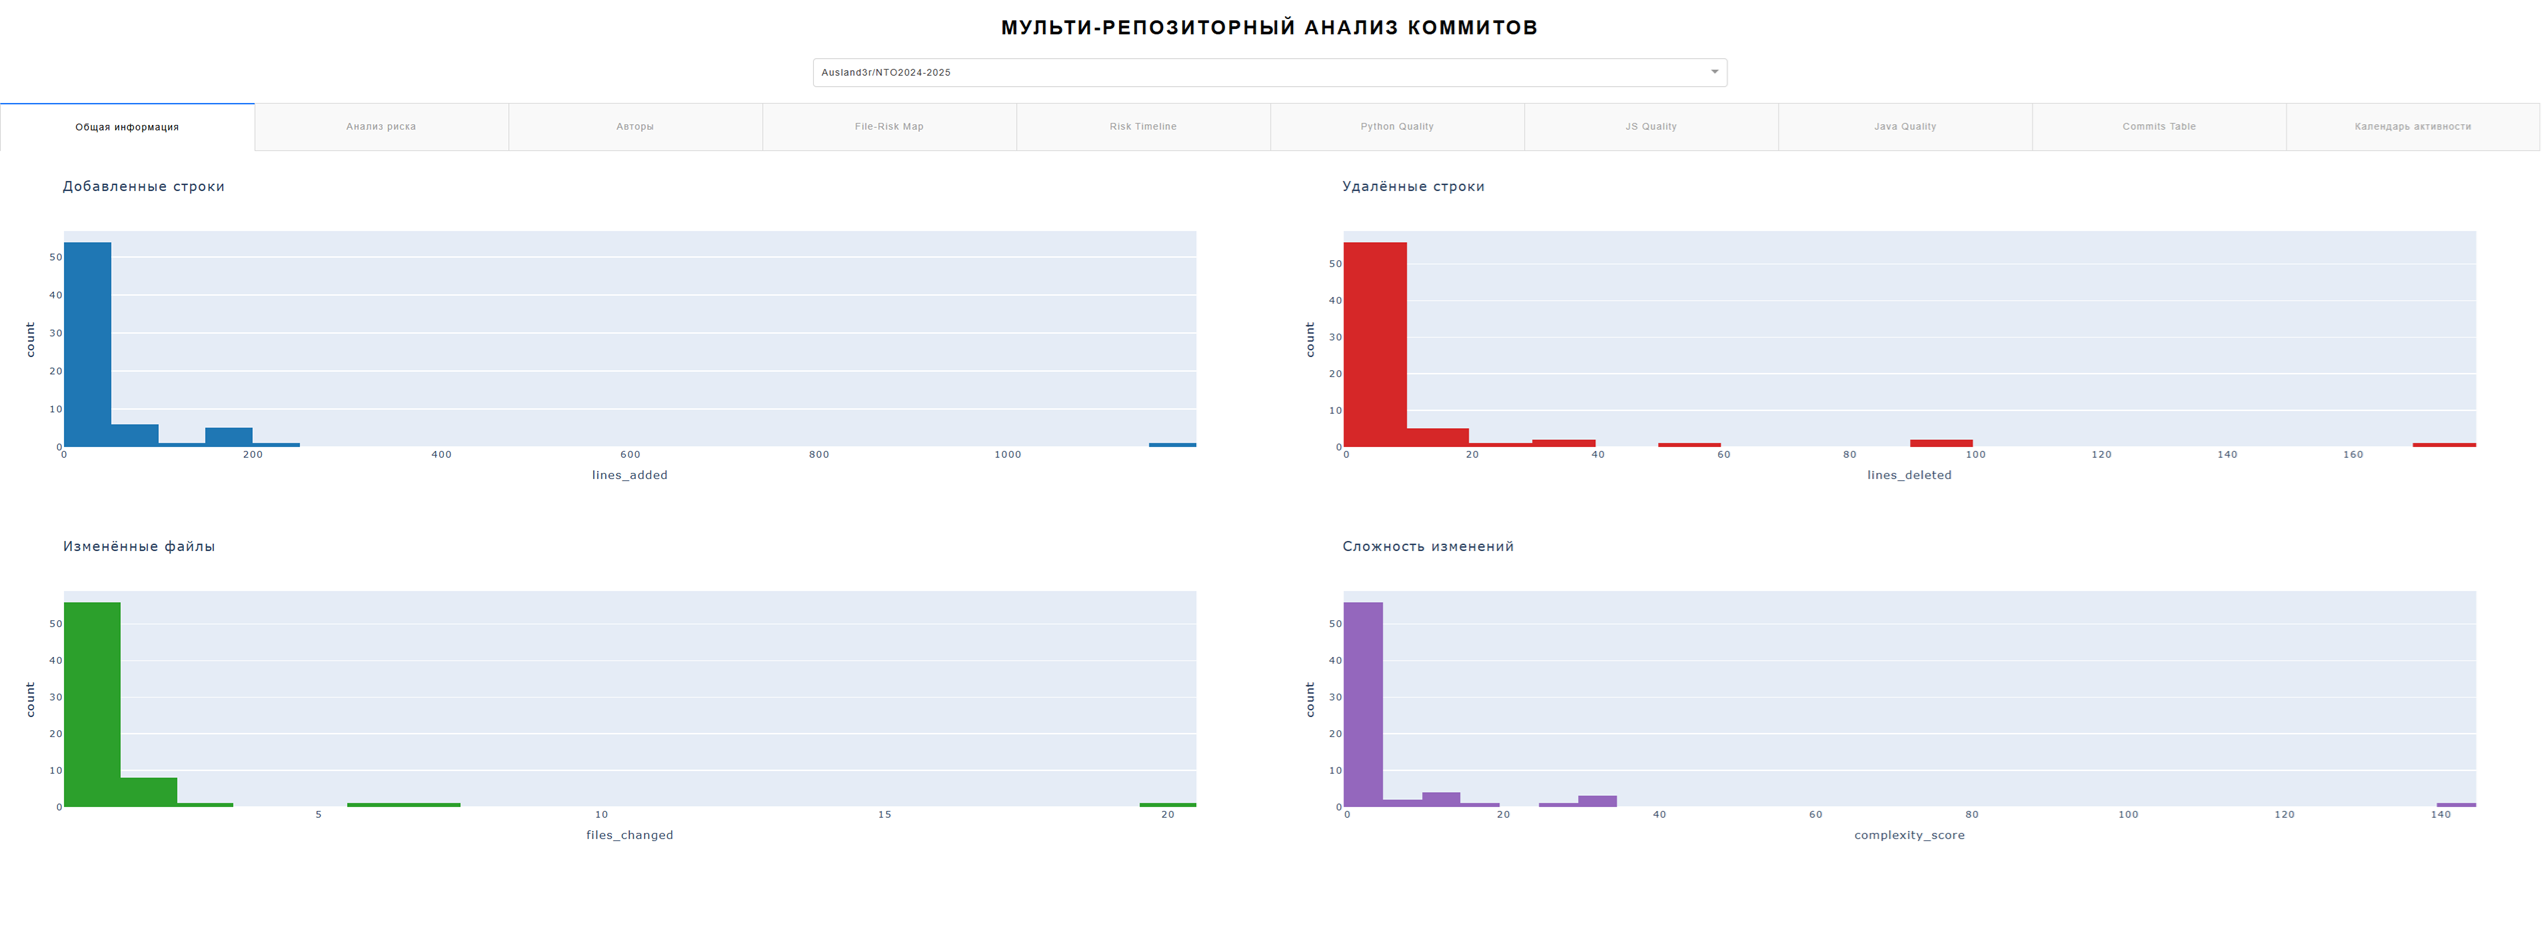
\includegraphics[width=\textwidth]{my_folder/images/first_page.png}
	\caption{Распределение изменений в коммитах: добавленные и удалённые строки, количество изменённых файлов и сложность изменений для проекта \texttt{Ausland3r/NTO2024-2025}.}
	\label{fig:commit_stats}
\end{figure}
На Рисунке~\ref{fig:risk_analysis} представлена информация об эффективности классификатора на этом репозитории. В таблице видим Precision=0.40, Recall=1.00, что соответствует метрикам модели на этих данных. Круговая диаграмма показывает, что около \verb|11.8%| коммитов отмечены как рисковые (красным цветом). Справа виден график «Risk vs Complexity»: наблюдается тенденция, что коммиты с большей сложностью имеют более высокий риск (жёлтым - рисковые коммиты). Данный анализ помогает подтвердить, что алгоритм верно выделяет несколько потенциально проблемных коммитов (в основном с большой сложностью), и диаграммы наглядно демонстрируют распределение рисковых изменений.

\begin{figure}[H]
	\centering
	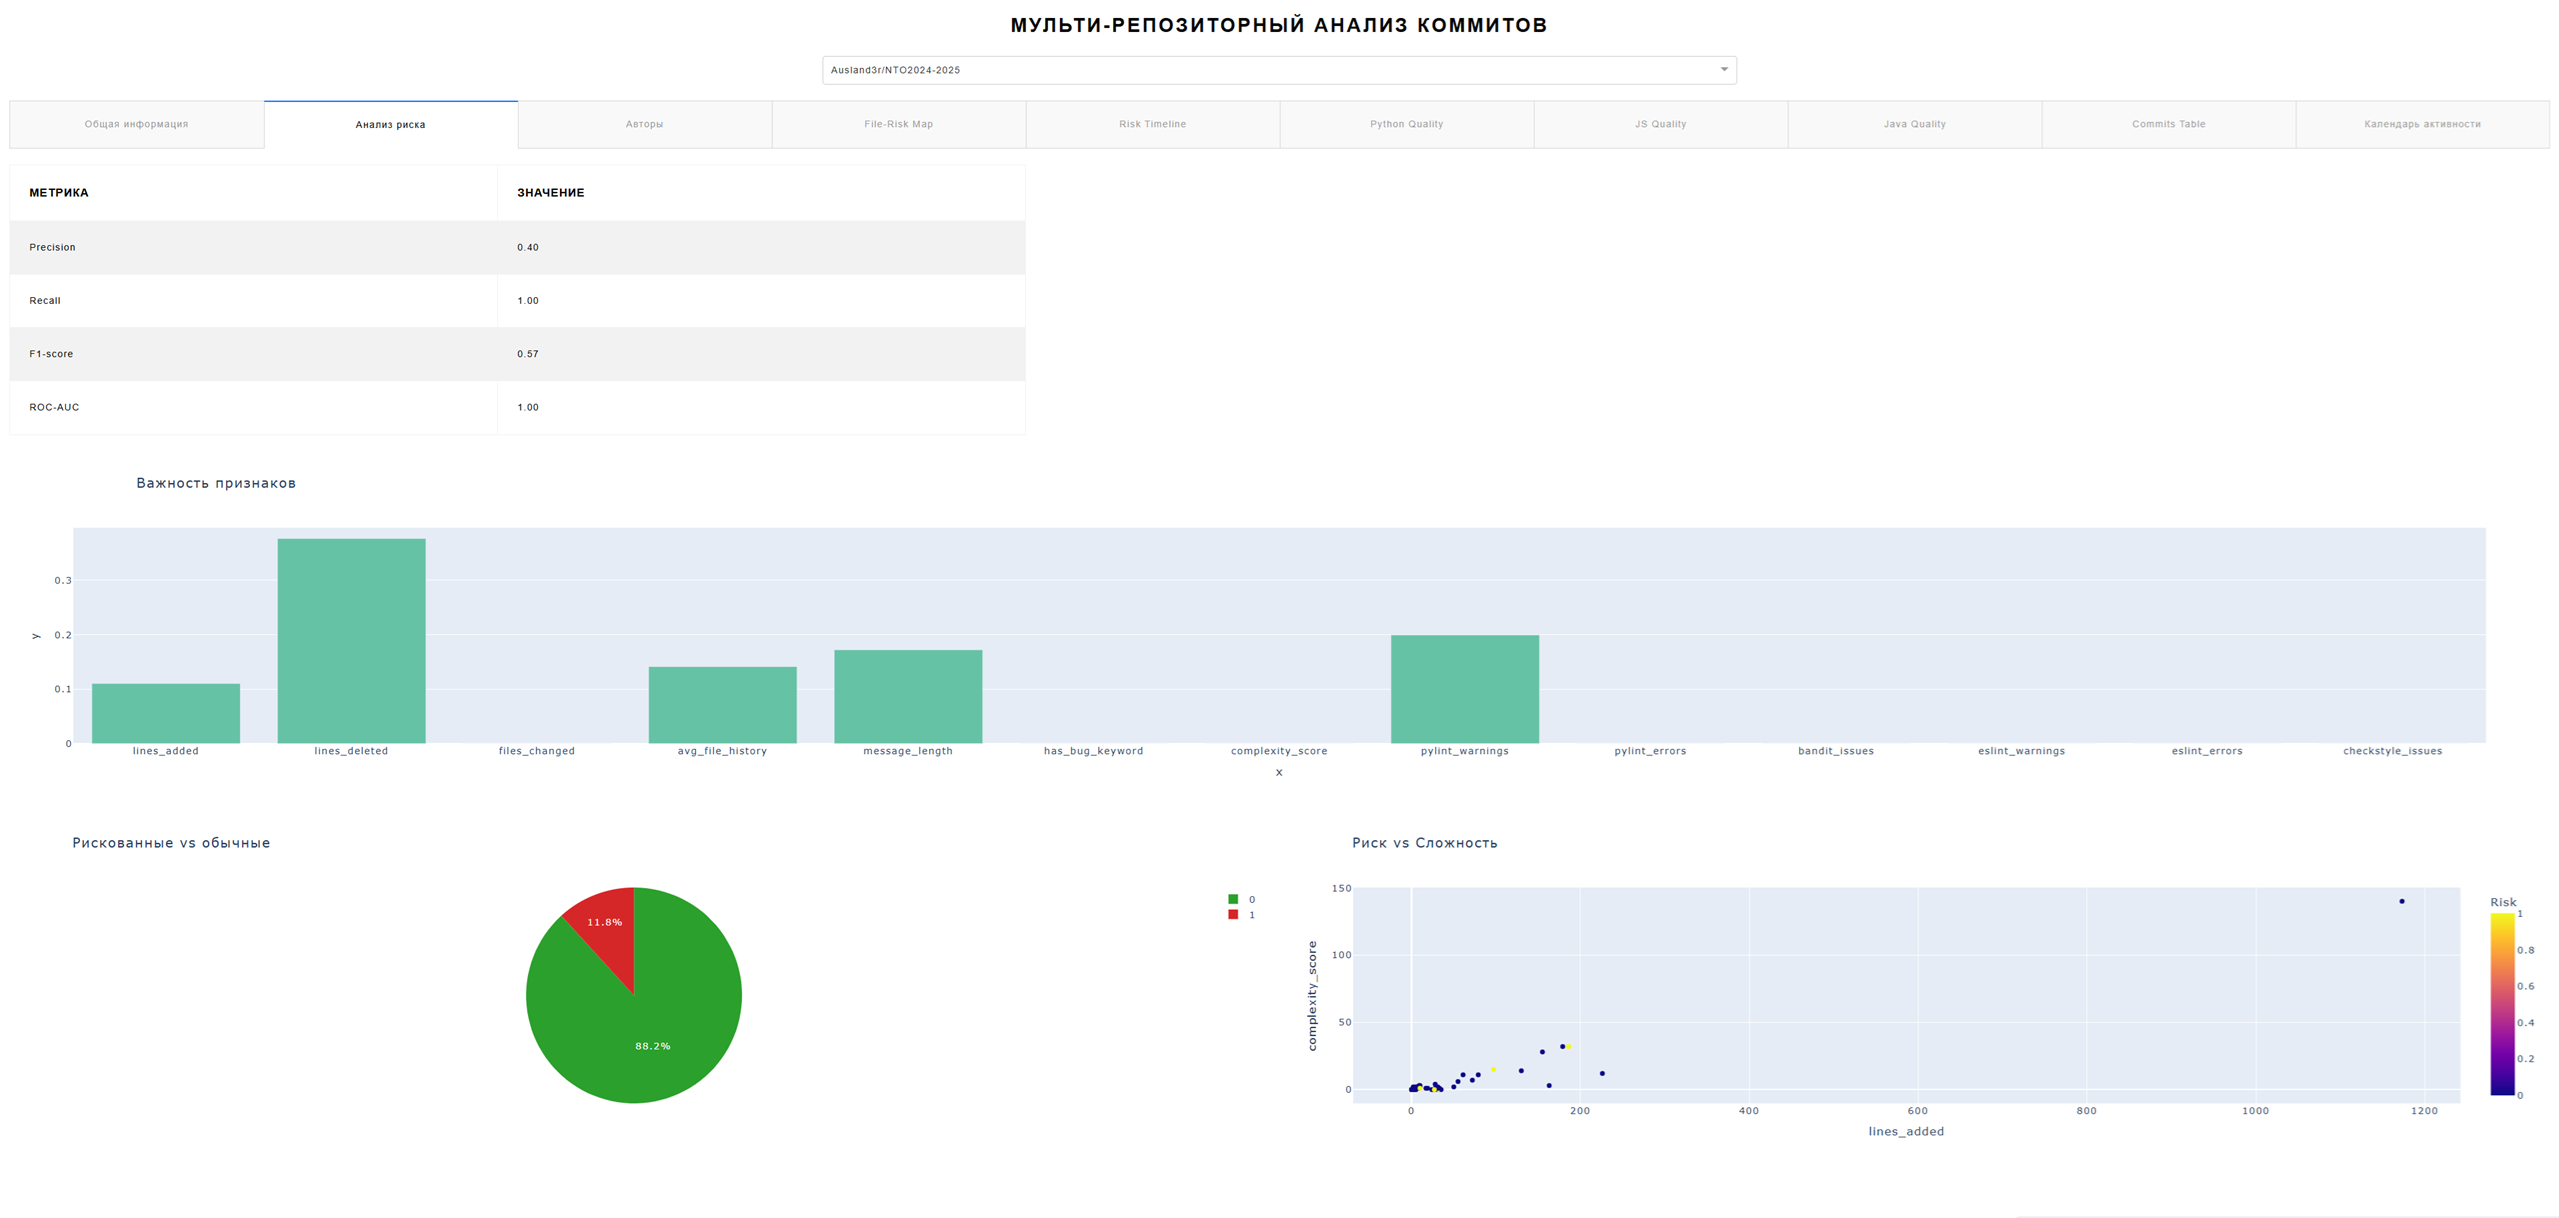
\includegraphics[width=\textwidth]{my_folder/images/second_page.png}
	\caption{Метрики классификации и распределение рисковых коммитов для репозитория \texttt{Ausland3r/NTO2024-2025}. Таблица показывает качество модели (Precision, Recall, F1, ROC-AUC), диаграмма слева — долю рисковых коммитов (красным), справа — зависимость риска от сложности.}
	\label{fig:risk_analysis}
\end{figure}

Рисунок~\ref{fig:authors} иллюстрирует вклад разных разработчиков. Слева видно, что основной объём коммитов внесли \texttt{Ausland3r} и \texttt{DenisovDmitrii} (по ~30 коммитов каждый), остальные авторы — единичные вклады. Справа график показывает средний риск по автору: например, \texttt{Fliegende\_Rehe} (средний риск ~0.4) выделяется как относительный «рисковый» автор, хотя у него было меньше коммитов. Такая визуализация помогает в определении, кто из участников при текущем анализе вносит больше потенциально проблемных изменений.

 \begin{figure}[ht]
	\centering
	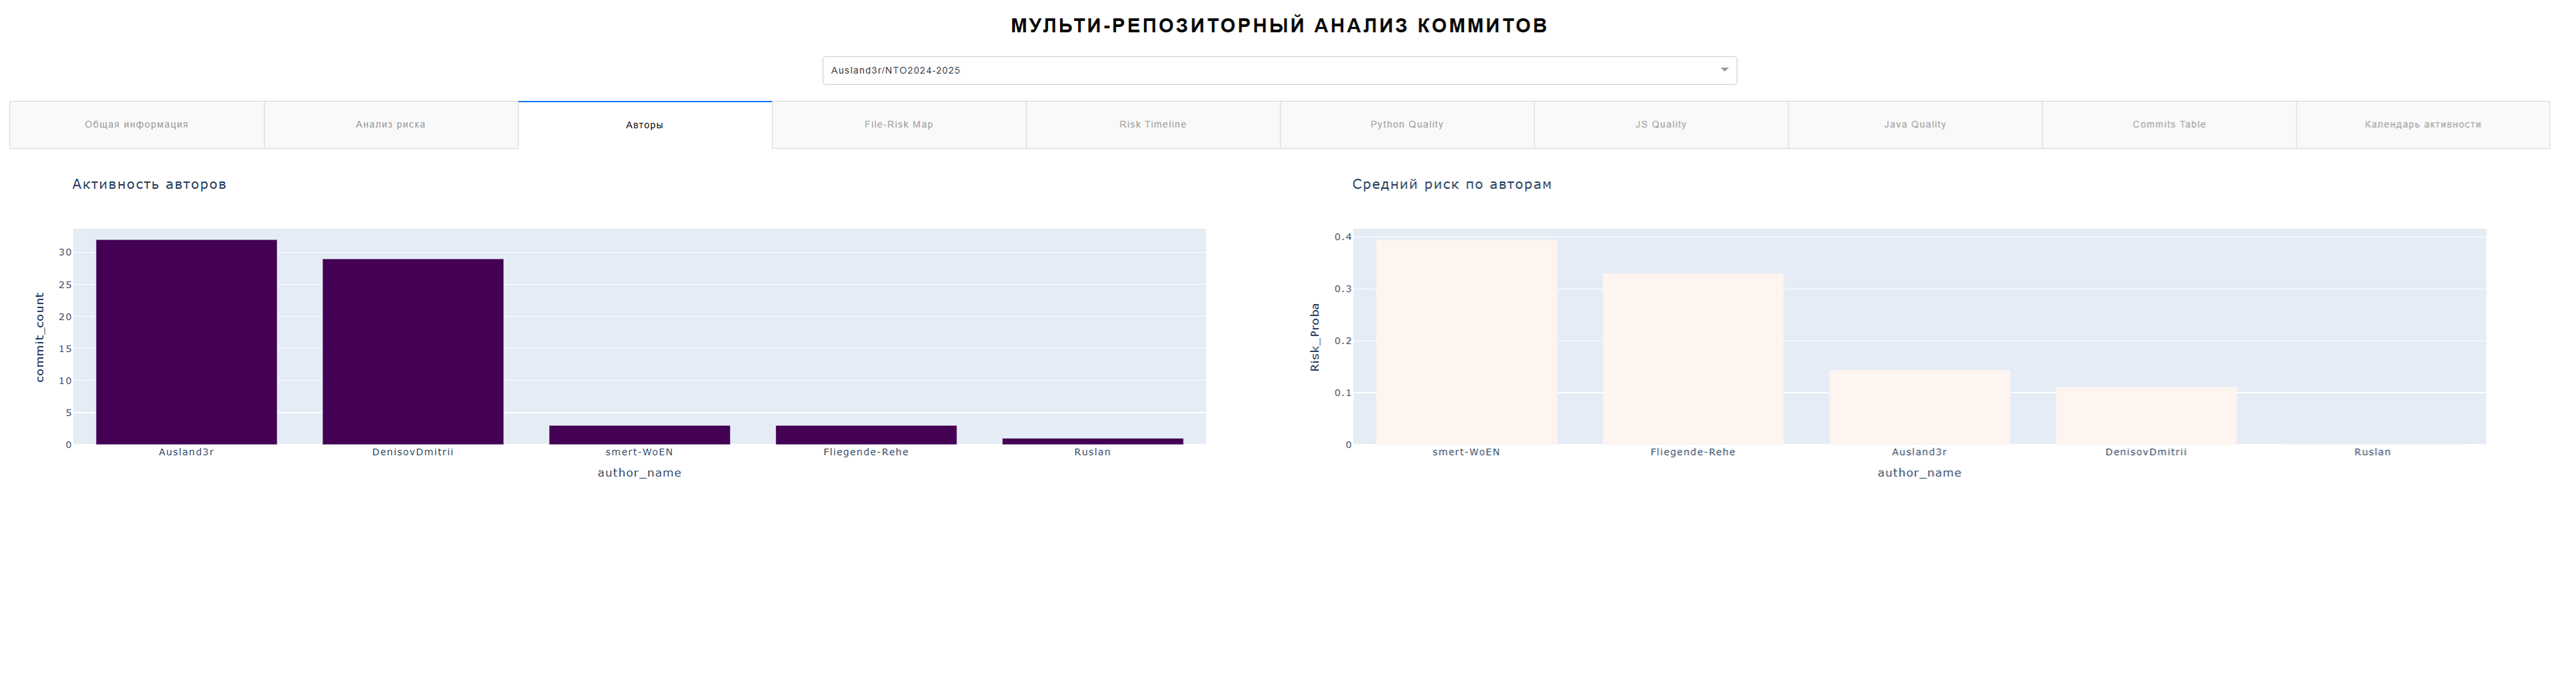
\includegraphics[width=\textwidth]{my_folder/images/third_page.png}
	\caption{Активность авторов и средний риск на автора для проекта \texttt{Ausland3r/NTO2024-2025}. Слева — число коммитов на автора, справа — усреднённый риск.}
	\label{fig:authors}
\end{figure}
 \begin{figure}[ht]
	\centering
	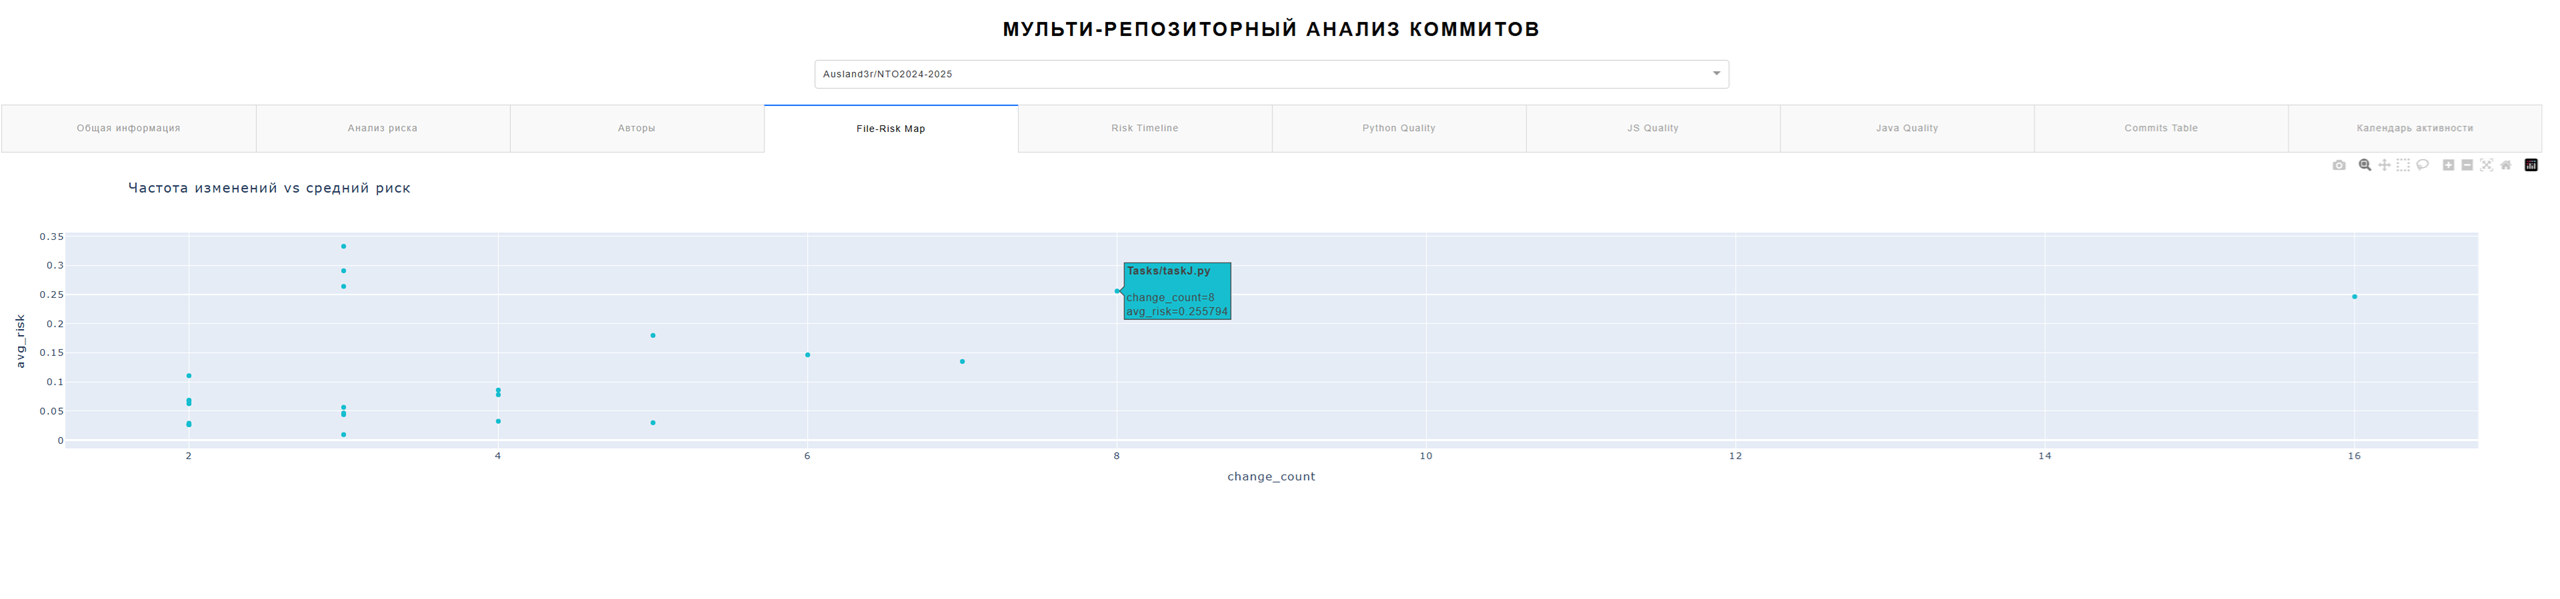
\includegraphics[width=\textwidth]{my_folder/images/forth_page.png}
	\caption{Файловая карта риска (частота изменений vs средний риск) для \texttt{Ausland3r/NTO2024-2025}. Точка \texttt{Task/taskJ.py} выделена как файл с 8 изменениями и средним риском 0.25.}
	\label{fig:file_risk}
\end{figure}

На Рисунке~\ref{fig:file_risk} представлена файловая карта: по горизонтали — число изменений файла (\texttt{change\_count}), по вертикали — средний риск изменений этого файла. Замечено, что файл \texttt{Task/task1.py} менялся 8 раз и имеет средний риск ~0.38 (отмечен на графике). Большинство же файлов имеют низкий риск. 

Такая диаграмма позволяет выявлять «горячие точки» проекта — файлы, часто изменяющиеся и с высоким риском, требующие внимания. 


Наконец, Рисунок~\ref{fig:timeline} демонстрирует динамику проекта. По синей линии видно, что средний риск коммитов постепенно рос с ноября 2024 по декабрь 2024. В мае 2025 на проекте снова были внесены изменения. Оранжевые столбцы отображают количество предупреждений статического анализа во времени. Видно несколько пиков предупреждений в начале проекта; далее они стабилизировались на низком уровне. Такая временная диаграмма подчёркивает, как со временем изменялась стабильность проекта, и позволяет своевременно заметить всплески риска или предупреждений. В целом приведённые визуализации показывают, что проект велся относительно аккуратно. 



\begin{figure}[ht]
	\centering
	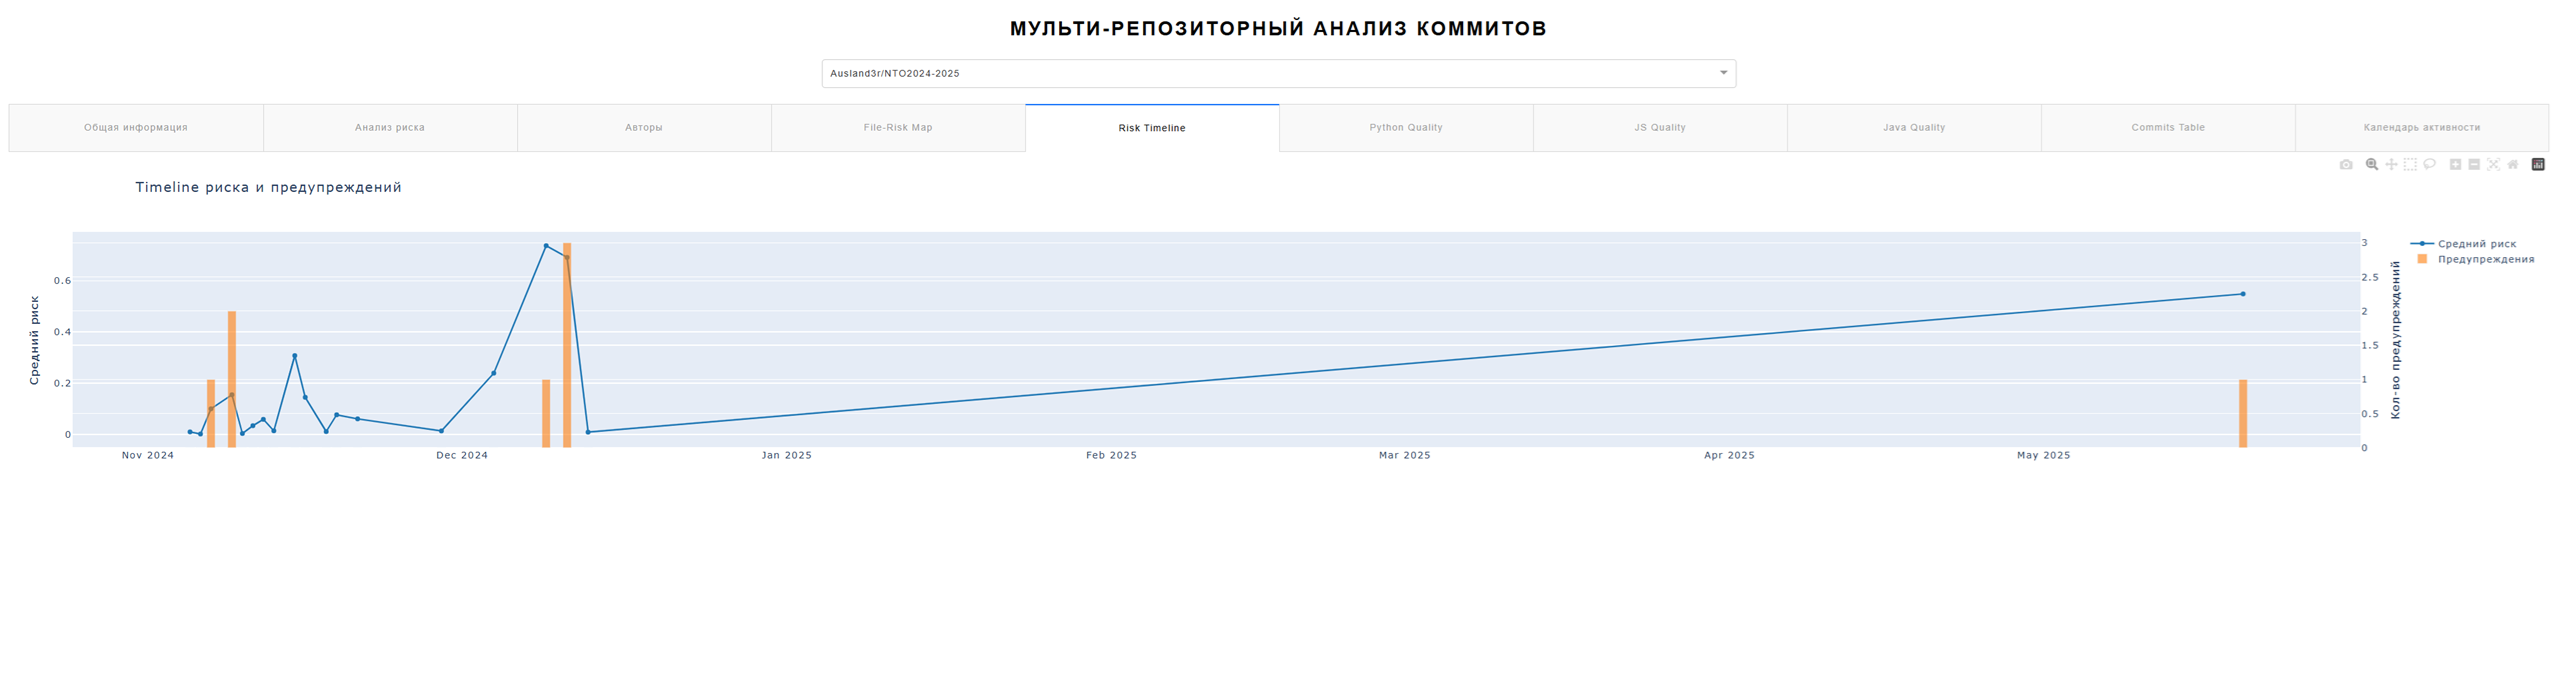
\includegraphics[width=\textwidth]{my_folder/images/fifth_page.png}
	\caption{Временная шкала риска и предупреждений для \texttt{Ausland3r/NTO2024-2025}. Синяя линия — средний риск коммитов с течением времени, оранжевые столбцы — число предупреждений статического анализа.}
	\label{fig:timeline}
\end{figure}

Визуальные представления, такие как вышеперечисленные, существенно упрощают анализ состояния проекта: они помогают быстро выделить проблемные области (рисковые коммиты, ответственные авторы, модифицируемые файлы и т.д.), которые трудно заметить при простом чтении логов. Аналитическая панель с такими графиками позволяет команде разработки эффективнее контролировать качество кода и прогнозировать потенциальные риски. 

\subsection{Описание страницы рекомендаций по коммитам}

На данной странице отображаются рекомендации по каждому коммиту репозитория, сгенерированные на основе анализа риска и метрик изменений. Рекомендации призваны помочь разработчикам и ревьюерам быстро оценить потенциальные проблемы и принять соответствующие меры.

\begin{figure}[ht]
	\centering
	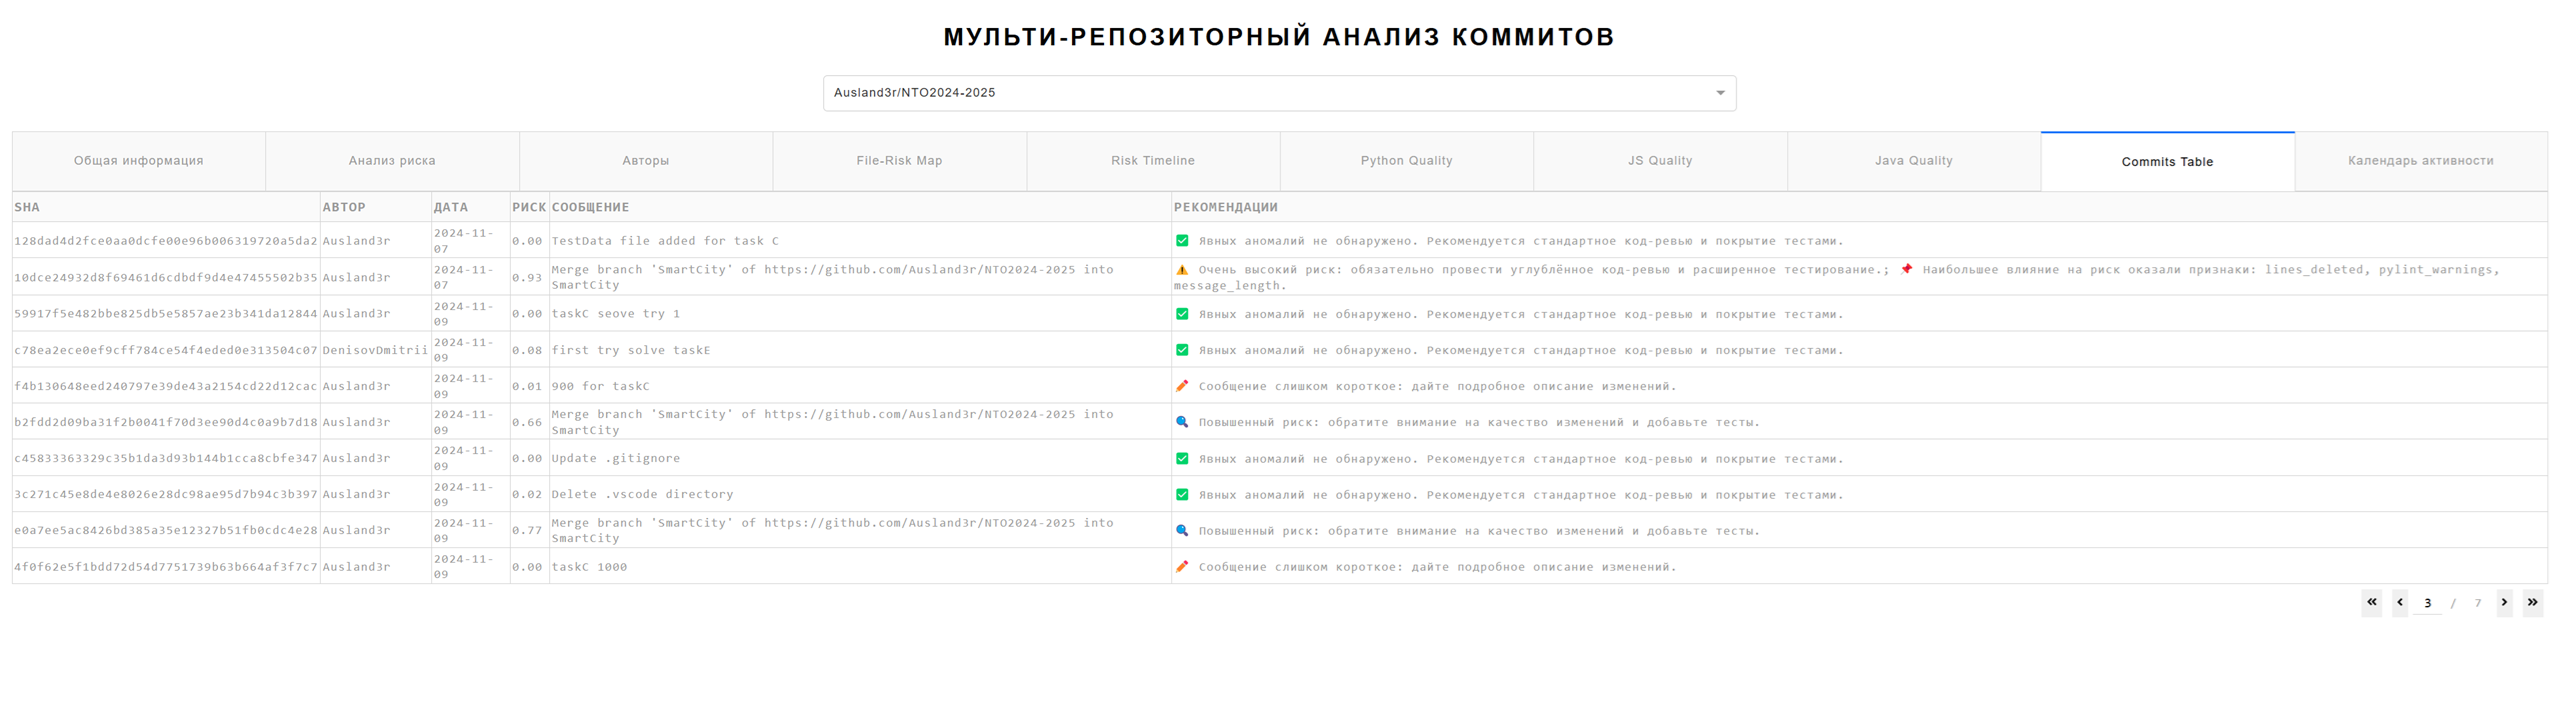
\includegraphics[width=\textwidth]{my_folder/images/capa_page.png}
	\caption{Таблица рисков и предупреждений для \texttt{Ausland3r/NTO2024-2025}.}
	\label{fig:timeline123}
\end{figure}

Основные виды рекомендаций включают:

\begin{itemize}
	\item Высокий риск (например, вероятность риска выше 0.8): 
	\begin{itemize}
		\item Рекомендуется углублённое код-ревью и расширенное тестирование.
		\item При наличии — показаны наиболее значимые признаки, повлиявшие на оценку риска, чтобы понять причины высокой оценки.
	\end{itemize}
	\item Повышенный риск (риск в диапазоне 0.5–0.8): 
	\begin{itemize}
		\item Совет обратить внимание на качество изменений и добавить тесты.
	\end{itemize}
	\item Качество сообщения коммита:
	\begin{itemize}
		\item Сообщения с длиной менее 15 символов получают рекомендацию расширить описание изменений.
		\item Очень длинные сообщения (более 200 символов) предлагается структурировать или сократить.
	\end{itemize}
	\item Объём изменений:
	\begin{itemize}
		\item Если количество изменённых строк значительно превышает среднее по репозиторию (свыше среднего плюс два стандартных отклонения), рекомендуется разбивать изменения на более мелкие логические части.
	\end{itemize}
	\item Специфические сигналы:
	\begin{itemize}
		\item Коммиты с ключевыми словами, указывающими на исправление багов, сопровождаются рекомендацией проверить наличие регрессионных тестов и обновление документации.
	\end{itemize}
\end{itemize}

Реализация рекомендаций основана на анализе различных метрик коммита, таких как длина сообщения, объём изменений, количество изменённых файлов, а также вероятности риска, вычисленные моделью. Это позволяет делать выводы не только на основе простых пороговых значений, но и учитывать специфику репозитория (через статистики по проекту) и значимость отдельных признаков риска.

Таким образом, представленные рекомендации реально соответствуют конкретному коммиту и его характеристикам, помогая в раннем выявлении потенциальных проблем и улучшении процесса код-ревью.

\vspace{0.5em}
Пример рекомендаций по коммиту:

\begin{quote}
	\begin{itemize}
		\item Очень высокий риск: обязательно провести углублённое код-ревью и расширенное тестирование.
		\item  Наибольшее влияние на риск оказали признаки: lines\_deleted, pylint\_warnings, message\_length.
		\item  Сообщение слишком короткое: дайте подробное описание изменений.
		\item Объём изменений (150) значительно превышает среднее (50.3). Разбейте коммит на более мелкие логические части.
	\end{itemize}
\end{quote}

Такая система рекомендаций повышает прозрачность оценки качества коммитов и способствует улучшению практик разработки в команде.

\section{Выводы}
В результате экспериментального тестирования подтверждена корректность реализации разработанной системы: интерфейс и функциональные блоки работают согласно заданию, а обученный классификатор рисковых коммитов показывает адекватные метрики на реальных данных. Успешно протестирована модель генерации рекомендаций CAPA: выявленные рекомендации соответствуют ожидаемым паттернам исправлений. Модульные тесты покрыли основные пути выполнения, включая граничные сценарии, что свидетельствует о надёжности кода. Нагрузочные тесты показали, что система масштабируема — даже при анализе тысячи коммитов реакция остаётся предсказуемой, хотя оптимизации статического анализа целесообразны для ускорения. Сильными сторонами подхода являются комплексность анализа (объединение статики кода, анализа коммитов и визуализации) и высокая адаптивность модели (универсальный класс классификатора позволяет легко тестировать новые алгоритмы). Подробные визуализации дают мощный инструмент мониторинга проекта. Возможные улучшения: расширение набора признаков за счёт динамических метрик (например, метрики сборки или покрытия тестами), а также использование реальных размеченных данных для обучения классификатора вместо эвристической псевдоразметки. При дальнейшем развитии можно добавить автоматические рекомендации по приоритетам исправлений на основе выявленных рисков. В целом, проведённое экспериментальное тестирование подтвердило, что разработанный подход позволяет эффективно выявлять и анализировать рисковые изменения в репозиториях, обеспечивая корректность работы системы и демонстрируя перспективу для дальнейшего улучшения инструментов разработки.